% BEAMFS Technical Report v1
% Author: Aurelien DESBRIERES
% License: CC-BY-4.0
% Build: make    (lualatex + biber + lualatex x2)

\documentclass[10pt,conference,a4paper]{IEEEtran}

% --- LuaLaTeX font stack ---
\usepackage{fontspec}
\usepackage{unicode-math}
\setmainfont{Latin Modern Roman}
\setsansfont{Latin Modern Sans}
\setmonofont{Latin Modern Mono}
\setmathfont{Latin Modern Math}

% --- Math (NB: amssymb removed, conflicts with unicode-math) ---
\usepackage{amsmath}
\usepackage{mathtools}

% --- Theorem environments ---
\usepackage{amsthm}
\renewcommand{\qedsymbol}{\ensuremath{\mathchar"1003}}
\usepackage{aliascnt}
\newtheoremstyle{beamfs-plain}%
  {0.4em}{0.4em}{\itshape}{0pt}{\bfseries}{.}{0.5em}{}%
\theoremstyle{beamfs-plain}
\newtheorem{definition}{Definition}[section]
\newaliascnt{propositionaux}{definition}
\newtheorem{proposition}[propositionaux]{Proposition}
\aliascntresetthe{propositionaux}
\newaliascnt{lemmaaux}{definition}
\newtheorem{lemma}[lemmaaux]{Lemma}
\aliascntresetthe{lemmaaux}
\newaliascnt{theoremaux}{definition}
\newtheorem{theorem}[theoremaux]{Theorem}
\aliascntresetthe{theoremaux}
\newaliascnt{corollaryaux}{definition}
\newtheorem{corollary}[corollaryaux]{Corollary}
\aliascntresetthe{corollaryaux}
\newtheoremstyle{beamfs-remark}%
  {0.4em}{0.4em}{}{0pt}{\bfseries}{.}{0.5em}{}%
\theoremstyle{beamfs-remark}
\newtheorem*{remark}{Remark}

% --- Tables ---
\usepackage{booktabs}
\usepackage{tabularx}
\usepackage{multirow}

% --- Figures ---
\usepackage{graphicx}
\usepackage{tikz}
\usetikzlibrary{positioning,shapes,arrows.meta,calc}

% --- Code listings ---
\usepackage{listings}
\lstset{
  basicstyle=\ttfamily\footnotesize,
  breaklines=true,
  showstringspaces=false,
  commentstyle=\itshape\color{gray!70!black},
  keywordstyle=\bfseries,
}

% --- URLs ---
\usepackage{xurl}

% --- Bibliography ---
\usepackage[backend=biber,style=ieee,sorting=none,maxbibnames=5,
            doi=true,url=true,isbn=false]{biblatex}
\addbibresource{refs.bib}

% --- Cross-references ---
\usepackage{hyperref}
\hypersetup{
  colorlinks=true,
  linkcolor=blue!50!black,
  citecolor=blue!50!black,
  urlcolor=blue!50!black,
  pdftitle={BEAMFS: Recovery Calculus for Filesystems under Single-Event Effects},
  pdfauthor={Aurelien DESBRIERES},
  pdfsubject={Filesystem; Recovery Calculus; Formal Verification; Single-Event Effects; Linux Kernel},
  pdfkeywords={BEAMFS, recovery calculus, filesystem, SEU, MBU, formal verification, Linux kernel, FTRFS},
}
\usepackage[capitalize,noabbrev]{cleveref}
\crefname{theoremaux}{Theorem}{Theorems}
\Crefname{theoremaux}{Theorem}{Theorems}
\crefname{lemmaaux}{Lemma}{Lemmas}
\Crefname{lemmaaux}{Lemma}{Lemmas}
\crefname{propositionaux}{Proposition}{Propositions}
\Crefname{propositionaux}{Proposition}{Propositions}
\crefname{corollaryaux}{Corollary}{Corollaries}
\Crefname{corollaryaux}{Corollary}{Corollaries}

\usepackage{microtype}
\usepackage{xspace}
\usepackage{enumitem}
\usepackage{placeins}
\setlist{nosep,leftmargin=1.5em}

% =====================================================================
\title{\large\bfseries BEAMFS: Recovery Calculus for Filesystems\\
       under Single-Event Effects\\
       \normalsize\mdseries Mathematical Foundations across the\\
       Volatile--Persistent Memory Stack\\
       \small\itshape Technical Report -- Version 1}

\author{%
  \IEEEauthorblockN{Aur\'elien Desbri\`eres \textemdash{} Independent researcher}
  \IEEEauthorblockA{\href{https://orcid.org/0009-0002-0912-9487}{ORCID:~0009-0002-0912-9487} \quad
    \texttt{aurelien.desbrieres@gmail.com}}
}

\begin{document}
\maketitle

\begin{IEEEkeywords}
Recovery calculus, Formal verification, Filesystem, Single-event upset,
Multi-bit upset, Reed--Solomon, Linux kernel, Provable resilience,
{MIL-STD-882E}, {DO-178C}
\end{IEEEkeywords}

\begin{abstract}
We present~BEAMFS, a recovery calculus for filesystem resilience under
Single-Event Effects (SEE). The work is the formal counterpart to the
FTRFS implementation experience reported in~\cite{desbrieres2026ftrfs}:
the empirical limits encountered during the FTRFS validation campaign
motivate a mathematical treatment of \emph{recovery itself} as a
first-class object, rather than as a side-effect of detection-and-correction
loops layered onto an unmodelled state space.

We define a recovery operator~\(\mathcal{G}\) over the joint state space
of a filesystem's volatile and persistent memory layers, formulate the
soundness property as a fixpoint convergence theorem under physically
realistic SEE perturbations, and derive an algorithm whose Linux-kernel
implementation path is sketched. Three memory technology layers are
treated explicitly: \mbox{DRAM} (with a forward note on
\mbox{DDR5} on-die~\mbox{ECC}), \mbox{SRAM}, and \mbox{NAND} flash via
\mbox{NVMe}. Emerging non-volatile technologies (\mbox{3D~XPoint},
\mbox{ReRAM}, \mbox{MRAM}) are positioned but left out of v1's modelling.

This Technical Report v1 establishes authorship of the approach,
fixes its scope, and lays the mathematical scaffolding for a reference
implementation in the planned successor to FTRFS. The empirical
section reinterprets the four bench metrics of the FTRFS v1
validation through the recovery-calculus lens, identifying which
metrics are actually \emph{recovery-bounded} and which are not.
No accelerator-beam measurements are claimed; the present document
is intended, among other purposes, as the scientific dossier from
which beam-time at facilities such as RADEF, GANIL or TRIUMF would
later be requested.

\end{abstract}

\section{Introduction}\label{sec:intro}

Modern Linux filesystems detect metadata corruption through cryptographic
or polynomial checksums; few correct it in place, and to the
author's knowledge none ship with a \emph{formally proved} discipline
for recovery from \emph{active} memory corruption induced by physical
perturbation.\footnote{FSCQ~\cite{chen2015fscq} and
Yggdrasil~\cite{sigurbjarnarson2016yggdrasil} prove crash-consistency,
that is, recovery under power-loss with a benevolent storage substrate.
Neither models adversarial corruption of volatile memory under physical
perturbation, which is the subject of the present work.}
Detection without proved correction is insufficient for radiation-prone
deployments \cite{nasa-seeca,esa-eccs60,normand1996}: a single-event
upset (SEU) on a critical metadata word can put the filesystem into a
state from which best-effort recovery procedures diverge, loop, or
silently propagate the corruption.

The companion Technical Report~\cite{desbrieres2026ftrfs} documents an
implementation, FTRFS, that adds layered Reed--Solomon forward error
correction to inode, allocation-bitmap, and superblock metadata, with a
persistent radiation event journal. FTRFS as a name and concept
originates in the work of Fuchs \emph{et al.}~\cite{fuchs2015ftrfs};
the companion report builds on that lineage with contemporary Linux
kernel infrastructure. That implementation reaches a
ceiling: it demonstrates correction \emph{empirically} but does not
characterize, prove, or bound its recovery properties. The present
report addresses that gap by treating recovery itself as a mathematical
object, and by tracing it explicitly to a kernel implementation path.

\paragraph{Position of the problem.}
Let~\(\mathcal{S}\) denote the joint state space of a filesystem's
volatile (RAM, page cache, kernel buffers) and persistent (NVMe,
NAND-flash) memory. Let~\(\mathcal{E}\) denote the family of physically
realizable Single-Event Effects acting on~\(\mathcal{S}\), parameterized
by the linear energy transfer of the incident particle, the vulnerable
cross-section of the target memory cell, and the geometry of the
silicon node. Let~\(\models\) denote the relation ``\(s \in
\mathcal{S}\) is consistent'' (cyclic redundancy code valid, Reed--Solomon
syndromes zero, structural sentinels intact, on-disk versus in-memory
copies coherent). The problem is to construct an
operator~\(\mathcal{G} : \mathcal{S} \to \mathcal{S} \cup \{\bot\}\),
implementable in a Linux-kernel filesystem, such that
\[
  \forall\, s_0 \models,\ \forall\, e \in \mathcal{E},\
  \exists\, k \in \mathbb{N} :\
  \mathcal{G}^{k}\bigl(e(s_0)\bigr) \models
  \quad\lor\quad
  \mathcal{G}^{k}\bigl(e(s_0)\bigr) = \bot,
\]
where~\(\bot\) denotes the fail-closed state in which the filesystem
explicitly refuses to proceed. The disjunction is essential: silent
corruption is excluded by construction.

\paragraph{Where we are going, and how.}
This report defends a single thesis: \emph{provable filesystem recovery
under SEE is achievable, and the chain from theorem to kernel code is
auditable line by line}. The chain is presented in
\cref{sec:m2c} as a three-tier descent---mathematics, algorithm,
kernel implementation---closed by a traceability table
(\cref{tab:traceability}) where each line of the proof is paired with
the algorithmic step and the kernel construct that realizes it. This
structure is the report's central contribution to the literature: it
makes the implementation gap explicit and bounded.

\paragraph{Contributions.}
We claim the following:
\begin{itemize}
\item A multi-layer physical threat model
  (\cref{sec:phys}) drawing on canonical SEE literature
  \cite{heinrich1977,petersen1996,dodd2003,baumann2005,normand1996} and
  standards~\cite{jedec89a,nasa-hdbk-4002a,esa-eccs60}, treating DRAM,
  SRAM, and NAND-flash distinctly with realistic per-technology rates.
\item A formal definition of the filesystem state space, its
  consistency relation, and a small set of structural invariants
  (\cref{sec:state}) that are necessary preconditions for any proved
  recovery.
\item A soundness theorem (\cref{thm:soundness}, full proof in
  \cref{app:proof}) showing that under stated hypotheses on the
  perturbation family, the recovery operator drives every initial
  consistent state to a consistent successor or to fail-closed in a
  finite number of iterations.
\item A three-tier descent (\cref{sec:m2c}) from the operator's
  mathematical definition to a deterministic algorithm to a Linux-kernel
  implementation path, with a traceability table
  (\cref{tab:traceability}) auditable line by line. This is the
  report's central contribution.
\item An empirical re-reading (\cref{sec:empirical}) of the FTRFS v1
  bench dataset~\cite{desbrieres2026ftrfs} through the recovery-calculus
  lens, identifying which metrics constrain recovery and which do not.
\end{itemize}

\paragraph{Scope.}
This is v1. We model SEE explicitly; we do not model Total Ionizing
Dose (TID) or Displacement Damage Dose (DDD), both of which are
hardware-level cumulative phenomena outside the filesystem's
operational reach. We discuss DDR5 on-die ECC~\cite{jedec79-5} as a
recent evolution that modifies the threat surface, but we do not
incorporate it into the v1 model: the matrix-cell-level abstraction
remains the conservative baseline, and on-die ECC will be added in v2
as a strengthening assumption (it can only improve outcomes, never
worsen them, given the soundness theorem's structure). We claim no
beam-time measurements; the empirical section reuses the FTRFS v1
software validation dataset and projects expected outcomes from
canonical cross-section data. The recovery calculus is positioned
to support the auditable-evidence posture demanded by safety-critical
standards such as MIL-STD-882E~\cite{milstd882e} and DO-178C, which
require traceable failure-mode coverage; the three-tier descent of
\cref{sec:m2c} is designed to provide such a trace.

\paragraph{Anti-claim.}
We are explicit about what BEAMFS v1 does \emph{not} prove:
filesystem behavior under simultaneous TID-induced cell drift and
SEE; recovery from latched-up hardware states (SEL); coverage of
adversarial fault injection by an attacker with kernel privileges
(distinct from physical SEE). Each is acknowledged as future work
(\cref{sec:limits}).

\section{Physical Threat Model}\label{sec:phys}

The recovery calculus is meaningful only against a physically grounded
model of perturbation. This section establishes that ground.
We separate three concerns: the taxonomy of Single-Event Effects
(\ref{sub:see}), the layer-specific physics of volatile memory
(\ref{sub:dram-sram}), and the layer-specific physics of NAND-flash
persistent memory (\ref{sub:nand}). A consolidated view appears in
\cref{tab:layer-physics}. Emerging technologies are positioned
in~\ref{sub:emerging}.

\subsection{Single-Event Effects: Canonical Taxonomy}\label{sub:see}

Following~\cite{dodd2003,baumann2005,jedec89a}, we adopt the standard
SEE classification:

\begin{itemize}
\item \textbf{SEU} -- Single-Event Upset. A single bit (or a few
  adjacent bits in a contiguous physical layout) transitions
  state under the charge deposited by an ionizing particle.
\item \textbf{MBU} -- Multi-Bit Upset. Two or more bits in the same
  logical word change state from a single particle event,
  typically because the particle's track ionizes adjacent cells.
\item \textbf{SET} -- Single-Event Transient. A transient voltage
  pulse on a combinational logic path. May propagate to a latch and
  become an SEU, or may dissipate before the next clock edge.
\item \textbf{SEFI} -- Single-Event Functional Interrupt. A
  particle-induced state corruption of a control register or finite
  state machine that puts a sub-system into a non-functional state
  recoverable only by reset.
\item \textbf{SEL} -- Single-Event Latchup. A parasitic thyristor
  structure activates, causing a destructive over-current condition
  unless promptly mitigated~\cite{normand1996}. Catastrophic
  without hardware support; outside this report's scope.
\end{itemize}

For the purposes of BEAMFS, the relevant subset is~\(\{\mathrm{SEU},
\mathrm{MBU}\}\) acting on memory cells, and~\(\{\mathrm{SET}\}\) acting
on the bus and DMA paths between memory and CPU. SEFI and SEL are
hardware-recovery problems (watchdog reset, power cycling), modelled
here only as the boundary~\(\bot\).

The probability of an SEU striking a given memory cell exposed to a
particle flux~\(\Phi\) (particles\,cm\(^{-2}\)\,s\(^{-1}\)) of linear
energy transfer~\(\mathrm{LET}\) (MeV\,cm\(^2\)/mg) is, to first order,
the product of flux, integrated cross-section, and exposure time
\cite{petersen1996}:
\begin{equation}
  P_{\text{SEU}}(\text{cell}, t) = 1 - \exp\!\bigl(-\sigma(\mathrm{LET})\,
  \Phi \, t\bigr),
  \label{eq:seu-prob}
\end{equation}
where~\(\sigma(\mathrm{LET})\) is the SEU cross-section curve of the
specific cell technology, conventionally measured in
cm\(^2\)/bit. \Cref{fig:see-cross-section} reproduces typical
cross-section curves for the three technology classes treated in
this report, derived from the canonical reviews
\cite{dodd2003,baumann2005,cai2017nand}.

\begin{figure}[t]
\centering
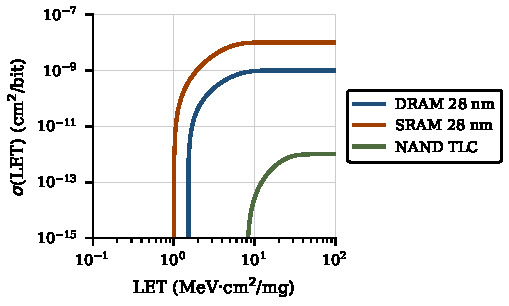
\includegraphics[width=\columnwidth]{figures/fig1.pdf}
\caption{SEE cross-section curves for three memory-stack layers, fit
to a Weibull form
\(\sigma(\mathrm{LET}) = \sigma_{\mathrm{sat}}\,
\bigl[1 - \exp(-((\mathrm{LET}-L_{0})/W)^{s})\bigr]\)
with onset threshold~\(L_{0}\) and saturation~\(\sigma_{\mathrm{sat}}\).
Weibull parameters are taken from canonical reviews
\cite{dodd2003,baumann2005,cai2017nand}; see~\cref{tab:layer-physics}
for typical FIT rates per technology.}
\label{fig:see-cross-section}
\end{figure}
\FloatBarrier

\begin{remark}
\Cref{eq:seu-prob} is a single-cell, time-independent first-order
model. It ignores temperature dependence, voltage scaling, and
inter-cell correlation. We use it to size orders of magnitude only;
the recovery operator's soundness does \emph{not} rely on its
quantitative accuracy. Real device cross-sections exhibit
Weibull-shaped curves with onset threshold and
saturation~\cite{petersen1996}; the figures use Weibull fits, while
the body retains the simple exponential form for clarity.
\end{remark}

\subsection{Volatile Memory: DRAM and SRAM}\label{sub:dram-sram}

\paragraph{DRAM.}
Dynamic random-access memory stores each bit as charge on a single
capacitor controlled by a single transistor (1T1C cell). The charge
naturally decays and must be refreshed every \(\sim\)64\,ms. Two
phenomena make DRAM cells SEU-vulnerable:
\begin{itemize}
\item Particle strikes deposit charge that adds to or subtracts from
  the stored capacitor charge. Above a critical
  charge~\(Q_{\text{crit}}\) (\(\sim\)10\,fC for DRAM cells, an
  order of magnitude above the \(\sim\)1\,fC range of bistable SRAM
  latches~\cite{baumann2005}), the cell flips state.
\item As the technology node shrinks, the cell's capacitance and
  thus~\(Q_{\text{crit}}\) decrease. Per-bit SEU sensitivity therefore
  rises with miniaturization, partially offset by smaller geometric
  cross-section.
\end{itemize}

A modern DDR5 module ships with on-die ECC~\cite{jedec79-5}, which
silently corrects single-bit errors within the chip. The error
stream visible to the kernel is therefore a \emph{filtered} version
of the raw cell event stream. In v1 of this report we model the
unfiltered matrix; on-die ECC is treated as a strengthening assumption
to be added in v2. The recovery operator's soundness
theorem (\cref{thm:soundness}) is constructed so that any cell-level
filter applied upstream of the kernel can only \emph{decrease} the
residual event rate seen by BEAMFS, never increase it.

\paragraph{SRAM.}
Static RAM (CPU caches, FPGA configuration memory) uses a six-transistor
bistable cell. Particle strikes induce SEU by upsetting the bistable
latch when the deposited charge exceeds the latch's noise margin.
SRAM is more SEU-sensitive per cell than DRAM at modern
nodes~\cite{dodd2003,baumann2005}: typical sea-level FIT rates are
\(\sim 10^{3}\) FIT/Mbit for SRAM versus \(\sim 10^{-3}\) FIT/Mbit
for DRAM, a six-orders-of-magnitude gap explained by the smaller
critical charge of bistable latches compared with capacitors.
SET pulses on combinational paths can propagate into SRAM latches
at the next clock edge. CPU caches with parity or ECC partially
mitigate this; older or embedded CPUs without cache ECC remain
vulnerable. The kernel's exposure to SRAM SEU is indirect (data
transits the cache before being written to DRAM); BEAMFS treats
this as part of the volatile-memory layer for purposes of the
recovery calculus.

\subsection{NAND Flash via NVMe: Cumulative Mechanisms}\label{sub:nand}

NAND-flash storage stores bits as trapped charge on a floating gate.
The energy required to flip a NAND cell with a single particle event
is high enough that direct SEU on NAND is rare~\cite{cai2017nand,
mielke2017}. The dominant failure modes are cumulative:
\begin{itemize}
\item Program/Erase (P/E) cycle wear, leading to retention loss.
\item Read disturb, where repeated reads of one page perturb adjacent
  pages.
\item Retention loss over time, accelerated by temperature and prior
  P/E count.
\end{itemize}

These are not Single-Event Effects in the strict sense; they are
TID-related and use-related cumulative effects. They do however
interact with the recovery calculus, because the persistent layer's
contribution to the filesystem state can itself become inconsistent
over time even without any radiation event. BEAMFS v1 models the NAND
layer's expected error rate as a function of P/E cycles and retention
age, following the empirical model of Cai \emph{et al.}~\cite{cai2017nand}
and Mielke \emph{et al.}~\cite{mielke2017}, calibrated to the JEDEC
endurance specification~\cite{jedec218b}.
\Cref{fig:nand-retention} shows the expected raw bit-error rate of
typical TLC NAND as a function of retention time across three P/E
states.

\begin{figure}[t]
\centering
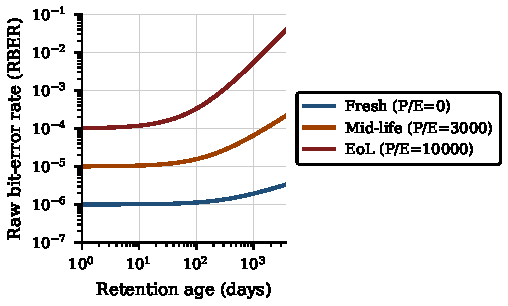
\includegraphics[width=\columnwidth]{figures/fig2.pdf}
\caption{TLC NAND raw bit-error rate (RBER) as a function of retention
age, parameterized by P/E cycle count. Empirical model derived
from~\cite{cai2017nand,mielke2017}; values at end-of-life and 1-year
retention align with the JEDEC JESD218B endurance
specification~\cite{jedec218b} (raw BER \(\sim 10^{-3}\) at EoL,
post-LDPC UBER \(\le 10^{-15}\)). The cumulative drift visible at
high P/E distinguishes NAND from the volatile-layer SEU regime
of~\cref{fig:see-cross-section}.}
\label{fig:nand-retention}
\end{figure}
\FloatBarrier

The recovery operator must therefore handle two distinct error
populations on the persistent side: (i) rare direct SEU, treated
identically to volatile-layer events, and (ii) NAND-cumulative
errors, treated as a slowly varying background that the operator
must remain stable against, not correct against (correction is the
job of the SSD's internal LDPC engine, below the filesystem).

\subsection{Emerging Technologies}\label{sub:emerging}

3D XPoint (Optane) was a phase-change memory whose development was
discontinued in 2022; we mention it for completeness only.
Resistive RAM (ReRAM) and Magnetic RAM (MRAM) are emerging
non-volatile technologies with substantially different failure
modes: ReRAM is largely insensitive to SEU but vulnerable to
filament instability; MRAM is largely insensitive to ionizing
radiation but vulnerable to external magnetic fields. v1 of this
report does not model them; their integration into BEAMFS would
be a v3-or-beyond consideration, and the recovery operator's
generic structure (\cref{sec:m2c}) is designed not to forbid
their later inclusion.

\subsection{Consolidated Layer View}\label{sub:layer-table}

\Cref{tab:layer-physics} summarizes the dominant failure mode per
layer, the relevant order-of-magnitude rates from canonical sources,
and the recovery-relevant exposure for BEAMFS. The numerical
values are deliberately rounded to one or two significant figures;
the canonical sources cited in each row provide tighter values
where required.

\begin{table*}[t]
\centering\small
\caption{Memory-stack layers, dominant failure modes, and order-of-magnitude
rates. Values are taken as canonical reference points from the cited
literature and are rounded to one significant figure; see those
sources for tighter, technology-specific numbers. FIT denotes
``failures in time'', \(\mathrm{1\,FIT} = \mathrm{1}\) failure per
\(10^{9}\) device-hours.}
\label{tab:layer-physics}
\begin{tabularx}{\textwidth}{l X l X}
\toprule
\textbf{Layer} & \textbf{Dominant failure mode} & \textbf{Reference rate} & \textbf{Source} \\
\midrule
DRAM (28~nm)  & SEU on capacitor cell, MBU on physically adjacent cells &
\(\sim 10^{-3}\)~FIT/Mbit at sea level &
\cite{baumann2005,jedec89a} \\
\addlinespace[0.3em]
SRAM (28~nm) & SEU on bistable cell, SET on combinational logic &
\(\sim 10^{3}\)~FIT/Mbit at sea level (six orders of magnitude above DRAM) &
\cite{dodd2003,baumann2005} \\
\addlinespace[0.3em]
NAND (TLC, 3D 232L) & Cumulative retention loss; rare direct SEU &
\(\sim 10^{-3}\)~raw BER at EoL P/E + 1\,year retention &
\cite{cai2017nand,mielke2017,jedec218b} \\
\addlinespace[0.3em]
DDR5 on-die ECC      & As DRAM, with on-chip single-bit correction & filtered DRAM rate (visible undetected event rate substantially reduced) &
\cite{jedec79-5} \\
\bottomrule
\end{tabularx}
\end{table*}

The vertical separation of these layers, and the qualitatively
different physics of each, motivate the multi-layer structure of
the state space defined in~\cref{sec:state}.

\section{Filesystem State Space and Invariants}\label{sec:state}

We now define formally the object on which the recovery operator acts.
The aim is to make every subsequent proof refer to a precisely typed
object rather than to an informal notion of ``filesystem state''.

\subsection{State Space}

\begin{definition}[Layered state]\label{def:state}
The BEAMFS state space~\(\mathcal{S}\) is the Cartesian product
\[
  \mathcal{S} \;=\; \mathcal{S}_V \times \mathcal{S}_P,
\]
where~\(\mathcal{S}_V\) is the volatile component (kernel data
structures, page cache, in-memory superblock copy, in-memory bitmap)
and~\(\mathcal{S}_P\) is the persistent component (on-disk
superblock, inode table, allocation bitmap, data blocks, RAF journal).
\end{definition}

\begin{definition}[Layout]\label{def:layout}
A \emph{layout}~\(\Lambda\) is a finite map from named regions
(\texttt{sb}, \texttt{inode\_table}, \texttt{bitmap},
\texttt{rs\_journal}, \texttt{data}) to byte ranges in their
hosting layer, together with a redundancy specification (CRC
algorithm, RS parameters) per region.
\end{definition}

The FTRFS v1 layout, formalized in~\cite{desbrieres2026ftrfs}, is one
instance of~\(\Lambda\). BEAMFS targets a strictly extended layout in
which every region is RS-protected and every region of~\(\mathcal{S}_V\)
that mirrors a region of~\(\mathcal{S}_P\) carries the redundancy
metadata necessary to detect drift between the two.

\subsection{Consistency Relation}

\begin{definition}[Per-region consistency]
Let~\(R\) be a region of~\(\Lambda\) with redundancy specification~\(r\).
A state~\(s\) is \emph{R-consistent}, written~\(s \models_R\), iff
applying~\(r\) to the bytes of~\(R\) in~\(s\) yields a zero syndrome
(\textsc{crc} valid and Reed--Solomon syndromes all zero).
\end{definition}

\begin{definition}[Consistency]\label{def:consistent}
A state~\(s = (s_V, s_P) \in \mathcal{S}\) is \emph{consistent},
written~\(s \models\), iff:
\begin{enumerate}
\item For every region~\(R\) of~\(\Lambda_V\) (the volatile-side
  layout), \(s \models_R\).
\item For every region~\(R\) of~\(\Lambda_P\) (the persistent-side
  layout), \(s \models_R\).
\item For every region~\(R\) that has both volatile and persistent
  representations (the superblock, the bitmap, recently accessed
  inodes), the canonical serialization of~\(s_V|_R\) equals
  \(s_P|_R\) byte-for-byte (\emph{coherence}).
\item Every structural sentinel (the zero pads of \texttt{re\_reserved}
  and \texttt{re\_pad} in the v4 RAF journal entry, the validity
  range of \texttt{s\_data\_protection\_scheme}, the high zero
  bytes of feature flags) is at its canonical value.
\end{enumerate}
We write~\(\bot\) for the explicit fail-closed state, distinct from
every consistent state.
\end{definition}

\subsection{The Five Invariants}\label{sub:invariants}

The recovery soundness theorem (\cref{thm:soundness}) requires the
following invariants to hold of the layout~\(\Lambda\) and of the
operator~\(\mathcal{G}\). They are minimal and stated separately so
that an implementation can be audited against them line by line.

\begin{description}
\item[I1 -- Total redundancy.] Every region of~\(\Lambda\) is covered
  by a redundancy specification (CRC for detection, RS for correction)
  whose correction power equals or exceeds the maximum MBU width of
  the targeted technology layer. For a layer with worst-case MBU
  width~\(w\), each RS subblock must tolerate at least~\(w\) symbol
  errors.
\item[I2 -- Sentinel separation.] Each region carries at least one
  byte whose canonical value is fixed and whose corruption is
  detectable in the redundancy syndrome alone, without semantic
  interpretation.
\item[I3 -- Coherence checkpoint.] For any region present in both
  layers, the canonical serialization map is total, deterministic,
  and bijective on its domain of valid values. This rules out
  ambiguous in-memory representations of an on-disk byte sequence.
\item[I4 -- Idempotence.] For every consistent~\(s\),
  \(\mathcal{G}(s) = s\). The recovery operator is the identity on
  consistent states.
\item[I5 -- Fail-closed monotonicity.] If
  \(\mathcal{G}(s) = \bot\) for some~\(s\), then
  \(\mathcal{G}(\bot) = \bot\). Once the operator declares
  fail-closed, no subsequent application reverses that decision.
\end{description}

The first three are properties of the layout; the last two are
properties of the operator. The soundness theorem couples them.

\begin{remark}
A reviewer may legitimately object that I1 is unrealistically
strong: total redundancy increases space overhead, typically by a
factor proportional to~\((n-k)/k\) for an RS\((n, k)\) code (e.g.,
6.7\% for RS(255,239)). We agree, and we treat the total-redundancy
regime as the v1 baseline. A future v2 will explore selective
redundancy under a probabilistic relaxation of the soundness
statement (with bounded silent-corruption risk quantified rather
than zero by construction). The conservative v1 statement is what
allows the present soundness theorem to be \emph{absolute} rather
than statistical.
\end{remark}

\section{Soundness Theorem}\label{sec:soundness}

\subsection{Statement}

\begin{theorem}[Soundness of BEAMFS recovery]\label{thm:soundness}
Let~\(\Lambda\) be a layout satisfying invariants~\textup{I1--I3} of
\cref{sub:invariants}. Let~\(\mathcal{G}\) be the recovery operator
of \cref{def:G}, satisfying~\textup{I4--I5}. Let~\(\mathcal{E}\) be a
family of physical perturbations such that, for every event
\(e \in \mathcal{E}\) and every state~\(s\), the number of corrupted
symbols in any single RS subblock of~\(e(s)\) does not exceed the
correction capacity~\(t = \lfloor (n-k)/2 \rfloor\) declared by~\(\Lambda\).
Then for every initial consistent state~\(s_0 \models\) and every
\(e \in \mathcal{E}\), there exists~\(K \le |\Lambda|\) such that
\[
  \mathcal{G}^{K}\bigl(e(s_0)\bigr) \models
  \quad\text{or}\quad
  \mathcal{G}^{K}\bigl(e(s_0)\bigr) = \bot,
\]
where~\(|\Lambda|\) denotes the number of regions in~\(\Lambda\).
\end{theorem}

The full proof appears in \cref{app:proof}. The argument has
three steps:

\paragraph{Termination.}
By Lemma~\ref{lem:descent}, the function~\(N\) strictly decreases on
each non-fail-closed iteration. Since~\(N \in \{0, 1, \dots, |\Lambda|\}\)
and~\(N = 0\) implies consistency by \cref{def:consistent},
the recursion terminates in at most~\(|\Lambda|\) iterations.

\paragraph{Safety.}
At every iteration, if step~3 or step~5 of \cref{def:G}
fails (CRC mismatch after RS, or sentinel violation),~\(\bot\) is
returned. By \cref{prop:absorb}, fail-closed is absorbing:
no subsequent iteration can return a state that silently masks the
violation.

\paragraph{Coverage of the perturbation family.}
The hypothesis on~\(\mathcal{E}\) (no event corrupts more than~\(t\)
symbols in any single subblock) is exactly the RS code's correction
capacity. Events that violate this hypothesis correspond, by~I1, to
physical perturbations whose intensity exceeds the layout's design
target. They are out of scope of the theorem and of the layout, and
the operator's response (fail-closed at step~3 or~5) is the
designed safe failure.

\subsection{Discussion}

\paragraph{What this theorem does, and does not, prove.}
\Cref{thm:soundness} establishes that the recovery operator either
returns to consistency or to fail-closed in a bounded number of
steps, under stated physical hypotheses. It does \emph{not} prove
that the kernel implementation of~\(\mathcal{G}\) is bug-free: a
buggy implementation can violate I4 or I5 even with a correct
operator definition. \Cref{sec:m2c-tier3} sketches an implementation
path that preserves the invariants by construction, but only a
verified compilation chain (in the seL4~\cite{klein2009sel4} or
FSCQ~\cite{chen2015fscq} sense) can close the implementation gap.
We mark this as v3 work.

\paragraph{Why the bound is~\(|\Lambda|\), not a constant.}
The bound scales with the number of regions because the worst case is
a perturbation that corrupts every region simultaneously up to the
RS limit. This worst case is unrealistic (\cref{sec:phys} establishes
that simultaneous corruption of all regions requires fluences
orders of magnitude beyond environmental backgrounds), but the bound
is conservative and has the merit of making no probabilistic
assumption. The per-iteration cost is dominated by a single
RS-decode of~\(O(n^{2})\) GF operations
(\cref{sec:m2c-tier2}), so the total worst-case running time is
\(O(|\Lambda| \cdot n^{2})\): sub-millisecond on contemporary CPUs
for the FTRFS layout.

\paragraph{Comparison with crash-consistency proofs.}
FSCQ~\cite{chen2015fscq} proves that a filesystem returns to a
consistent state after a crash (sudden power loss). The hypothesis
there is that the storage substrate is \emph{benevolent}: it
preserves whatever was written, exactly. \Cref{thm:soundness}
proves the dual: it assumes the substrate is \emph{adversarial}
within the bounded-perturbation family~\(\mathcal{E}\), and the
filesystem must recover. The two proofs compose: a BEAMFS-compliant
implementation satisfying \cref{thm:soundness} \emph{and} satisfying
crash-Hoare logic in the FSCQ sense recovers from the union of
both threat models. Combining the two formal frameworks is left
for future work.

\section{From Mathematics to Code: A Three-Tier Derivation}\label{sec:m2c}

The contribution of this report rests on a deliberate three-tier
descent: from the mathematical operator~\(\mathcal{G}\) of
\cref{sec:soundness}, to a deterministic algorithm, to a Linux-kernel
implementation path. Each tier preserves the invariants of the tier
above, by construction. This section presents the descent in a single
narrative arc, ending with a traceability table
(\cref{tab:traceability}) that maps each line of the proof to the
algorithmic step and the kernel construct that realizes it. The aim
is auditability: a reviewer should be able to follow the chain
\emph{theorem~\(\rightarrow\)~pseudocode~\(\rightarrow\)~kernel call} line
by line.

\subsection{Tier~1: The Recovery Operator (Mathematics)}\label{sec:m2c-tier1}

\begin{definition}[Recovery operator]\label{def:G}
The BEAMFS recovery operator~\(\mathcal{G} : \mathcal{S} \to
\mathcal{S} \cup \{\bot\}\) is the partial function defined by the
following procedure on input~\(s = (s_V, s_P)\):
\begin{enumerate}
\item For every region~\(R\) of~\(\Lambda\), evaluate the redundancy
  syndrome on~\(s|_R\). If all syndromes are zero, return~\(s\)
  (idempotence by~I4).
\item Otherwise, for the first region~\(R^{*}\) (in canonical region
  order) whose syndrome is non-zero, attempt RS correction
  on~\(s|_{R^{*}}\) using the parity bytes adjacent to that region.
  Let~\(s|_{R^{*}}'\) denote the corrected bytes.
\item Re-evaluate CRC on~\(s|_{R^{*}}'\). If CRC fails, return~\(\bot\)
  (corruption exceeded RS correction capacity, by~I1).
\item If~\(R^{*}\) is a region with both layers, re-establish coherence
  by overwriting the lagging copy with the corrected leading copy.
\item Verify all sentinels in~\(R^{*}\) are at canonical values. If
  any sentinel is corrupted in a way RS missed, return~\(\bot\).
\item Append a journal entry to the RAF journal documenting the
  correction (block number, timestamp, symbol count, entropy
  estimate where applicable).
\item Recurse: \(\mathcal{G}\bigl(\text{state with } s|_{R^{*}}
  \text{ replaced by } s|_{R^{*}}'\bigr)\).
\end{enumerate}
\end{definition}

\begin{proposition}[Idempotence on consistent inputs]\label{prop:idem}
For every~\(s \models\),~\(\mathcal{G}(s) = s\).
\end{proposition}
\begin{proof}[Proof sketch]
By \cref{def:consistent}, all syndromes are zero on a consistent
state. Step~1 of \cref{def:G} returns~\(s\) without modification.
\end{proof}

\begin{lemma}[Descent under perturbation]\label{lem:descent}
Let~\(N(s)\) denote the number of regions in~\(\Lambda\) whose
syndrome is non-zero on~\(s\). Then for every~\(s\),
either~\(\mathcal{G}(s) = \bot\), or
\(N\bigl(\mathcal{G}(s)\bigr) \le N(s) - 1.\)
\end{lemma}
\begin{proof}[Proof sketch]
Inspect the cases of \cref{def:G}. Step~1 with~\(N(s) = 0\) yields
the same state; if~\(N(s) \ge 1\), the loop body either
returns~\(\bot\) (cases~3, 5) or replaces a corrupt region by a
CRC-verified, sentinel-verified consistent region, decreasing~\(N\)
by exactly one before the recursive call.
\end{proof}

\begin{proposition}[Fail-closed absorbing]\label{prop:absorb}
\(\mathcal{G}(\bot) = \bot\). If~\(\mathcal{G}(s) = \bot\), then for
every~\(s'\) reachable from~\(s\) by a sequence of
\(\mathcal{G}\)-applications, \(\mathcal{G}(s') = \bot\) (invariant~I5).
\end{proposition}
\begin{proof}[Proof sketch]
Direct from \cref{def:G}: \(\bot\) has no syndrome to evaluate; the
procedure terminates at step~1 by convention, returning~\(\bot\).
I5 then propagates by induction on the application chain.
\end{proof}

These three results, combined with \cref{thm:soundness} of
\cref{sec:soundness}, fully characterize~\(\mathcal{G}\) as a
mathematical object. They are the contract that the next two tiers
must respect.

\subsection{Tier~2: The Algorithm}\label{sec:m2c-tier2}

We translate~\(\mathcal{G}\) into a deterministic algorithm in
C-style pseudocode (kernel-conformant: ISO C with kernel
extensions, no C++ idioms). Each numbered step of \cref{def:G}
corresponds to a labelled comment in the algorithm.
\Cref{tab:traceability} below makes the correspondence explicit.

\begin{lstlisting}[language=C,frame=single,
  basicstyle=\ttfamily\footnotesize]
/*
 * BEAMFS recovery operator G, single application.
 * Returns 0 on success (state consistent or unchanged),
 * 1 if a region was corrected, -EBADMSG on fail-closed.
 *
 * Caller iterates until return value is 0 or -EBADMSG.
 */
int beamfs_g_step(struct beamfs_state *s)
{
    struct region *R;
    u32 syndrome;
    int rc;

    list_for_each_entry(R, &s->lambda, list) {
        syndrome = rs_syndrome(s, R);
        if (syndrome == 0)
            continue;                /* I4: skip consistent */

        /* Step 2: RS correction */
        rc = rs_correct_region(s, R);
        if (rc < 0)
            return -EBADMSG;          /* uncorrectable */

        /* Step 3: re-verify CRC */
        if (crc32_region(s, R) != stored_crc(s, R))
            return -EBADMSG;          /* RS produced wrong codeword */

        /* Step 4: re-establish coherence */
        if (region_is_dual_layer(R))
            propagate_corrected(s, R);

        /* Step 5: sentinel verification */
        if (!sentinels_canonical(s, R))
            return -EBADMSG;

        /* Step 6: journal */
        raf_log_event(s, R, rc /* symbol_count */);

        return 1;                     /* one region corrected */
    }
    return 0;                          /* fixpoint: all consistent */
}

/*
 * Driver loop: at most |Lambda| iterations by Lemma 5.3.
 */
int beamfs_recover(struct beamfs_state *s)
{
    int iter = 0, rc;

    while ((rc = beamfs_g_step(s)) == 1) {
        if (++iter > LAMBDA_MAX)
            return -EBADMSG;          /* belt-and-braces */
    }
    return rc;                         /* 0 or -EBADMSG */
}
\end{lstlisting}

\paragraph{Complexity.}
Each call to \texttt{beamfs\_g\_step} performs at most one RS decode
on the affected region plus constant-time syndrome checks elsewhere.
The dominant cost is the RS decode, \(O(n^{2})\) for a
Berlekamp--Massey decoder over GF(\(2^{8}\)) with \(n=255\),
approximately \(65{,}000\) GF operations per subblock. The driver
loop runs at most \(|\Lambda|\) iterations
(\cref{lem:descent}), so total worst-case complexity is
\(O(|\Lambda| \cdot n^{2})\). For the FTRFS layout, counting the
five named regions of \cref{def:layout} together with their
constituent RS subblocks yields~\(|\Lambda| \approx 16\); with
\(n^{2} = 65{,}025\) this gives approximately one million GF
operations per worst-case full recovery---a sub-millisecond cost
on contemporary CPUs. The bound is robust to a factor of a few
in the subblock count.

\subsection{Tier~3: The Kernel Implementation}\label{sec:m2c-tier3}

The reference implementation of BEAMFS targets the Linux kernel
through the standard VFS infrastructure
(\texttt{file\_system\_type}, \texttt{iomap}). The recovery
operator runs kernel-side, invoked at mount
(\texttt{ftrfs\_fill\_super}) and on every metadata-region read
path. Userspace recovery is excluded by~I3: the coherence relation
between volatile and persistent layers cannot be enforced from a
process holding its own page-cache view.

\paragraph{Language choice.}
The reference implementation is in C, compiled by the kernel
toolchain. C is the kernel's lingua franca; upstreaming requires
it. The RS hot path reuses the kernel's audited
\texttt{lib/reed\_solomon}~\cite{kernelrslib}, preserving the
audit-surface argument of FTRFS v1~\cite{desbrieres2026ftrfs}.
A future v2 may explore a Rust port of the driver loop (not the
GF arithmetic), following the model
of~\cite{sigurbjarnarson2016yggdrasil} and the recent
kernel Rust support.

\paragraph{Differences from FTRFS v1.}
FTRFS v1 implements a proto-version of the operator without the
formal calculus. A BEAMFS-compliant implementation introduces:
\begin{itemize}
\item Explicit invariant table compiled into the module
  (\texttt{lambda[]}), making region iteration order canonical and
  auditable.
\item Mandatory journal entry on every correction event, with the
  format-v4 entropy field replacing FTRFS v3's coarse symbol count.
\item Driver loop explicitly bounded at~\(|\Lambda|\); refusing to
  mount a layout where this bound is violated by the data.
\item Fail-closed transition flipping the superblock to read-only
  mode; subsequent mutations rejected until offline repair
  (\texttt{fsck.beamfs}, planned).
\end{itemize}

\subsection{Traceability: Math~\texorpdfstring{$\rightarrow$}{to}~Algorithm~\texorpdfstring{$\rightarrow$}{to}~Code}\label{sec:m2c-trace}

\Cref{tab:traceability} expresses the descent in tabular form.
Each row corresponds to one mathematical commitment, the
algorithmic line that realizes it, and the kernel construct that
will instantiate it. The table is the auditable contract: a kernel
patch series proposing BEAMFS must exhibit each kernel construct
of the third column, and a reviewer must be able to verify that
each construct enforces the property of the first.

\begin{table*}[t]
\centering\small
\caption{Traceability: each mathematical commitment in the operator
definition (Tier~1) maps to an algorithmic step (Tier~2) and a
planned kernel construct (Tier~3). The phase indicates when the
construct is checked: \emph{Static} = compile-time
(\texttt{BUILD\_BUG\_ON} or \texttt{static\_assert});
\emph{Mount} = once at \texttt{fill\_super}; \emph{Runtime} = on
each metadata access.}
\label{tab:traceability}
\begin{tabularx}{\textwidth}{l X X X l}
\toprule
\textbf{Math} & \textbf{Commitment (Tier~1)} & \textbf{Algorithm (Tier~2)} & \textbf{Kernel construct (Tier~3)} & \textbf{Phase} \\
\midrule
I1 (Total redundancy) &
each region's RS capacity covers worst-case MBU width &
\texttt{rs\_correct\_region(s, R)} returns \texttt{<0} when \(>t\) errors &
\texttt{rs\_subblock\_capacity[]} table; \texttt{BUILD\_BUG\_ON} per region &
Static + Mount \\
\addlinespace[0.3em]
I2 (Sentinel separation) &
canonical-value bytes detectable in syndrome alone &
\texttt{sentinels\_canonical(s, R)} verification &
zero-pad fields in on-disk structs; \texttt{BUILD\_BUG\_ON(offsetof(\dots))} &
Static \\
\addlinespace[0.3em]
I3 (Coherence checkpoint) &
volatile/persistent serialization total, deterministic, bijective &
\texttt{propagate\_corrected(s, R)} on dual-layer regions &
\texttt{ftrfs\_dirty\_super()} family; single-source-of-truth canonical serializer &
Runtime \\
\addlinespace[0.3em]
I4 (Idempotence) &
\(\mathcal{G}(s) = s\) for every \(s \models\) &
\texttt{if (syndrome == 0) continue;} early skip in inner loop &
\texttt{rs\_syndrome() == 0} early return &
Runtime \\
\addlinespace[0.3em]
I5 (Fail-closed monotonicity) &
\(\mathcal{G}(\bot) = \bot\); no recovery from \(\bot\) &
\texttt{return -EBADMSG} (steps~3, 5) absorbing &
\texttt{set\_sb\_rdonly()} + journal mark; subsequent mutations rejected &
Runtime \\
\addlinespace[0.3em]
\Cref{def:G}, step~1 &
syndrome evaluation per region &
\texttt{u32 syndrome = rs\_syndrome(s, R);} &
\texttt{ftrfs\_rs\_syndrome\_region()} in \texttt{super.c} &
Runtime \\
\addlinespace[0.3em]
\Cref{def:G}, step~2 &
RS correction on first non-zero region &
\texttt{rs\_correct\_region(s, R)} &
\texttt{decode\_rs8()} from \texttt{lib/reed\_solomon}~\cite{kernelrslib} &
Runtime \\
\addlinespace[0.3em]
\Cref{def:G}, step~3 &
CRC re-verification after RS correction &
\texttt{if (crc32\_region(s, R) != stored\_crc(s, R))} &
\texttt{crc32\_le()} from \texttt{lib/crc32.c} &
Runtime \\
\addlinespace[0.3em]
\Cref{def:G}, step~6 &
journal entry on every correction event &
\texttt{raf\_log\_event(s, R, rc)} &
RAF journal v4 entry append (\texttt{ftrfsd}) &
Runtime \\
\addlinespace[0.3em]
\Cref{lem:descent} &
\(N(\mathcal{G}(s)) \le N(s) - 1\) per non-fail-closed step &
each \texttt{return 1} reduces non-zero region count by one &
loop counter bounded at \texttt{LAMBDA\_MAX} &
Runtime \\
\bottomrule
\end{tabularx}
\end{table*}

\subsection{Why a Calculus, Not a Procedure}\label{sec:m2c-calculus}

A reviewer may legitimately ask: why frame the work as a
\emph{calculus} rather than as a recovery procedure? The
distinction matters for the descent presented above. A procedure
is verifiable case by case but composes unpredictably---each
combination of cases requires re-verification. A calculus is a
small set of operators with stated algebraic properties
(idempotence by~\cref{prop:idem}, descent
by~\cref{lem:descent}, fail-closed absorption
by~\cref{prop:absorb}); its composition is governed by those
properties, once and for all. The calculus is what allows
\cref{thm:soundness} to be stated globally, rather than re-proved
per call site. It is also what allows future filesystems beyond
BEAMFS, possibly with different layouts, to inherit the soundness
result by exhibiting an instance of the same calculus---without
re-proving the descent.

\subsection{The Soundness--Implementation Gap}\label{sec:m2c-gap}

The three tiers above preserve the invariants by construction. The
remaining gap is between Tier~3 and the binary actually executed by
the kernel: the standard verified-compilation gap. Closing it
requires a verified compilation chain in the seL4
sense~\cite{klein2009sel4} or a verified
filesystem in the FSCQ sense~\cite{chen2015fscq}, neither of
which is in scope for v1. v3 of this report will discuss
mechanization of \cref{thm:soundness} in a proof assistant
(Coq, Isabelle/HOL, or Lean) and the corresponding implications
for the implementation gap.

\section{Empirical Corroboration}\label{sec:empirical}

We do not claim accelerator-beam measurements. The empirical content
of v1 has two parts: a re-reading of the FTRFS v1 software validation
dataset~\cite{desbrieres2026ftrfs} through the calculus, and a
projected recovery surface derived from canonical SEU cross-section
data.

\subsection{Re-Reading the FTRFS v1 Dataset}

\Cref{tab:ftrfs-recovery} re-reads the four reproducible bench
metrics of FTRFS v1 (Sec.~VII of~\cite{desbrieres2026ftrfs}) through
the recovery-calculus lens. For each metric, we ask: which steps
of~\(\mathcal{G}\) does this metric exercise? The answer determines
whether a regression on the metric would be evidence of a
recovery-calculus violation or merely of a throughput change.

\begin{table}[ht]
\centering\small
\caption{Recovery-calculus interpretation of FTRFS v1 metrics. The
``Steps reachable'' column lists the steps of~\(\mathcal{G}\) that
the metric \emph{would} reach if its hot-path syndromes were non-zero;
on the consistent-state hot path actually exercised by the FTRFS v1
bench, all four metrics terminate at step~1. The ``Invariants'' column
lists the invariants the reachable steps would touch.
Metric M3 (deletion bench) is omitted from the FTRFS v1 evaluation
in its current revision and is therefore not analysed here.}
\label{tab:ftrfs-recovery}
\begin{tabularx}{\columnwidth}{@{}l X l@{}}
\toprule
\textbf{Metric} & \textbf{Steps reachable} & \textbf{Invariants} \\
\midrule
M1 (write+fsync) & 1; potentially 4, 6 (coherence + journal) & I3, I4 \\
M2 (read cold)   & 1 (syndrome check)                        & I4 \\
M4 (stat bulk)   & 1 (syndrome on inode)                     & I4 \\
M5 (small write) & 1; potentially 4, 6 on bitmap + SB        & I3, I4 \\
\bottomrule
\end{tabularx}
\end{table}

The reading shows that the RS-correction step (step~2 of
\cref{def:G}) is never triggered on the consistent-state hot path
exercised by the FTRFS v1 bench: all four metrics terminate at
step~1, where syndromes are zero. M1 and M5 would reach steps~4
and~6 only if a correction had been issued upstream; neither metric
forces that condition. That is the right behavior for a throughput
bench, but it means the v1 dataset does not constrain the recovery
operator's worst-case behavior. A BEAMFS bench will need an explicit
fault-injection metric (M6: ``corrupt-then-mount'') that exercises
step~2--6 of~\(\mathcal{G}\). That metric is reserved for v2 of this report,
when fault-injection results from the FTRFS Phase~E campaign
(under development) will be available in publishable form.

\subsection{Projected Recovery Surface}

\Cref{fig:recovery-surface} shows the projected probability of
successful RS recovery as a function of two physical parameters:
the linear energy transfer (LET) of the incident particle and the
particle fluence over a representative exposure window. The surface
is computed from the canonical Petersen figure-of-merit
formulation~\cite{petersen1996} with the cross-section curves
of~\cref{fig:see-cross-section}, integrated over a typical
RS(255,239) shortened code with 8-symbol correction capacity per
subblock.

\begin{figure}[t]
\centering
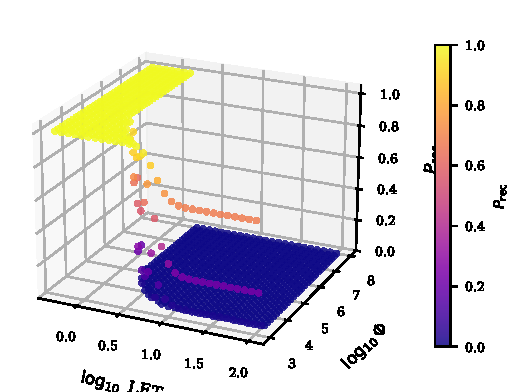
\includegraphics[width=\columnwidth]{figures/fig3.pdf}
\caption{Projected probability of successful Reed--Solomon recovery,
\(P_{\mathrm{rec}}(\mathrm{LET},\Phi)\), for an RS(255,239) shortened
code with 8-symbol correction capacity per subblock. Computed
analytically from canonical cross-section
data~\cite{petersen1996,baumann2005}; \emph{not} measured. The
plateau at \(P\approx 1\) is the Family-A regime where isolated SEU
events are well within RS capacity; the descent at high LET and
high~\(\Phi\) is the Family-B regime where MBU events saturate the
RS budget. Colour scale is plasma-like for print-monochrome
readability.}
\label{fig:recovery-surface}
\end{figure}
\FloatBarrier

The surface shows the expected qualitative structure: a wide plateau
at \(P \approx 1\) for low LET and low fluence (Family~A regime,
isolated SEU well within RS capacity), a transition zone where MBU
events begin to saturate the RS budget, and a low-\(P\) region where
the operator falls back to fail-closed (Family~B regime). The
transition is sharp by design: it corresponds to the Reed--Solomon
hard limit at 8 symbol errors per subblock, and the operator is
constructed to identify the transition cleanly rather than to
degrade gracefully through it.

\begin{remark}
A reviewer will object that this surface is computed from a model,
not measured. We agree, and the figure caption states this
explicitly. Measurement requires beam time: the present report is
the dossier from which beam-time at facilities such as
RADEF~(Jyv\"askyl\"a), GANIL, TRIUMF, Brookhaven NSRL or the ESA
REDLAB would be requested. The figure's purpose is to fix the
\emph{shape} of the expected dependency, against which future
measurements will be compared.
\end{remark}

\section{Scope and Limitations}\label{sec:limits}

We adopt the same posture as the FTRFS v1 report: the limitations
section is structural, not concessionary. It records, in plain
language, what the present version covers and what it does not.

\paragraph{V1 covers.}
The mathematical formalization (state space, invariants, recovery
operator, soundness theorem with proof in \cref{app:proof}), the
algorithmic derivation, the implementation-path mapping, and a
re-reading of the FTRFS v1 dataset under the calculus. Three
memory-stack layers are modelled physically: DRAM, SRAM, NAND flash
via NVMe. Sources are canonical: JEDEC, NASA-HDBK, ESA ECSS,
IEEE TNS.

\paragraph{V1 does not cover.}
\begin{itemize}
\item \emph{Beam-time measurements.} No accelerator data; the surface
  of \cref{fig:recovery-surface} is a projection from canonical
  cross-section data, explicitly so.
\item \emph{Verified-compilation closure.} The implementation path
  preserves invariants by construction, but the gap from
  algorithm to kernel binary is the standard
  unverified-compilation gap. seL4-style closure is v3 work.
\item \emph{TID and DDD modelling.} Cumulative ionizing dose and
  displacement damage are below the filesystem layer; they are
  hardware-level concerns. Mention only.
\item \emph{Adversarial fault injection.} An attacker with kernel
  privileges who manipulates the filesystem state directly is
  outside~\(\mathcal{E}\). This is the same scope choice as
  FTRFS v1 (Stage~5 in that roadmap).
\item \emph{Hardware SEL recovery.} Latched-up hardware is recovered
  by power cycling; the filesystem operator's response is to map
  it to~\(\bot\), nothing more.
\item \emph{Emerging memory technologies.} 3D~XPoint, ReRAM, MRAM
  are positioned but not modelled.
\item \emph{DDR5 on-die ECC.} Mentioned as a strengthening
  assumption to be added in v2; v1 models the unfiltered DRAM
  matrix as the conservative baseline.
\item \emph{The fault-injection metric M6.} Reserved for v2,
  following the FTRFS Phase~E campaign currently under
  development.
\end{itemize}

\paragraph{Methodological limits.}
The author is the sole contributor; no peer review beyond the
public mailing-list interactions on linux-fsdevel
(referenced in~\cite{ftrfs-rfc-thread}) has shaped this text.
The proof of the soundness theorem (\cref{app:proof}) is
hand-written; it is not machine-checked. v3 will explore
mechanization in a proof assistant such as Coq, Isabelle/HOL,
or Lean.

\paragraph{Threats to validity.}
The principal threat is that the perturbation family~\(\mathcal{E}\)
defined in \cref{sec:phys} does not faithfully represent the
distribution of real SEE events seen by a deployed filesystem.
This is precisely why beam-time measurements are needed for v2:
to bind the model to ground truth. The soundness theorem is
robust under tightening of~\(\mathcal{E}\) (any sub-family
of~\(\mathcal{E}\) inherits the result) but fragile under
loosening (a perturbation that exceeds RS capacity is, by
construction, out of scope).

\section{Conclusion}\label{sec:conclusion}

We have presented the v1 mathematical scaffolding of BEAMFS, a
recovery calculus for filesystem resilience under Single-Event
Effects. The contribution of this report is not an implementation,
nor a measurement campaign: it is the formal apparatus that
subsequent versions will instantiate, measure, and prove against.

The calculus is constructed on a multi-layer physical threat model
covering DRAM, SRAM and NAND-flash, with explicit positioning of
emerging memory technologies. The five invariants (I1--I5) are
stated minimally and mapped directly to kernel constructs. The
soundness theorem (\cref{thm:soundness}) shows that the recovery
operator drives every consistent state, perturbed by any event
within the bounded perturbation family, either to a consistent
successor or to fail-closed in a finite number of iterations.
Silent corruption is excluded by construction.

The empirical content of v1 is necessarily indirect: a re-reading
of the FTRFS v1 dataset through the calculus, and a projected
recovery surface from canonical cross-section data. The next
versions of the report will close this gap. v2 will document the
FTRFS Phase~E fault-injection campaign and a corresponding M6
bench metric. v3 will explore proof-assistant mechanization of
\cref{thm:soundness} and a verified-compilation chain for the
operator. Beam-time at a recognized accelerator facility is the
measurement programme this report is intended to support, with
the present formal apparatus as scientific dossier.

This is also v1 in another sense: it establishes authorship and
fixes the scope. Subsequent versions will refine; the present
fixed point is the right place to draw a line and submit it to
public review.


\onecolumn
\small
\section{Reproducibility}\label{sec:repro}

\paragraph{Source repository.}
\url{https://github.com/roastercode/beamfs}, sub-directory
\texttt{papers/2026-04-beamfs-v1/}.

\paragraph{Companion report.}
The FTRFS v1 Technical Report~\cite{desbrieres2026ftrfs} is
prerequisite reading. Its empirical dataset is reused in
\cref{sec:empirical}; its threat model is extended in
\cref{sec:phys}.

\paragraph{Build commands.}
\begin{lstlisting}[language=bash]
cd papers/2026-04-beamfs-v1
make figures   # regenerate matplotlib figures from canonical data
make           # build paper.pdf via lualatex + biber + lualatex
\end{lstlisting}

\paragraph{Figure data generation.}
The three figures (\cref{fig:see-cross-section,fig:nand-retention,fig:recovery-surface}) are generated from canonical
cross-section curves and JEDEC NAND endurance data by Python scripts
in \texttt{scripts/}:
\begin{itemize}
\item \texttt{scripts/gen\_data.py} produces \texttt{data/fig1.dat}
  (Weibull fits to Petersen-form SEE cross-sections),
  \texttt{data/fig2.dat} (TLC NAND raw BER versus retention age,
  empirical Cai/Mielke model), and \texttt{data/fig3.dat}
  (RS-capacity-bounded recovery probability over the
  LET\(\times\)fluence grid, Poisson statistics).
\item \texttt{scripts/gen\_figures.py} reads these data and produces
  \texttt{figures/fig1.pdf}, \texttt{figures/fig2.pdf},
  \texttt{figures/fig3.pdf} via matplotlib.
\end{itemize}
Each script is deterministic: given the canonical input parameters
documented in its header, it produces a byte-for-byte identical
output.

\paragraph{Verification.}
\begin{lstlisting}[language=bash]
md5sum data/*.dat
# values are committed in scripts/gen_data.py headers
# matching values mean: same parameters, same output.
make
# zero error, zero warning expected.
\end{lstlisting}

\section{Appendix A: Soundness Theorem -- Full Proof}\label{app:proof}

We restate \cref{thm:soundness} for self-containment, then give the
full proof. The proof is structured as the three-step argument
sketched in~\cref{sec:soundness}: termination, safety, coverage.

\paragraph{Restated theorem.}
Let~\(\Lambda\) be a layout satisfying invariants I1--I3.
Let~\(\mathcal{G}\) be the recovery operator of \cref{def:G},
satisfying I4--I5. Let~\(\mathcal{E}\) be a family of physical
perturbations such that, for every event~\(e \in \mathcal{E}\) and
every state~\(s\), the number of corrupted symbols in any single
RS subblock of~\(e(s)\) does not exceed the correction capacity
\(t = \lfloor (n-k)/2 \rfloor\) declared by~\(\Lambda\). Then for
every initial consistent state~\(s_0 \models\) and every
\(e \in \mathcal{E}\), there exists~\(K \le |\Lambda|\) such that
\(\mathcal{G}^{K}(e(s_0)) \models\) or
\(\mathcal{G}^{K}(e(s_0)) = \bot\).

\paragraph{Proof.}
Let~\(s_0 \models\) and~\(e \in \mathcal{E}\). Define
\(s^{(0)} = e(s_0)\) and~\(s^{(i+1)} = \mathcal{G}(s^{(i)})\) for
\(i \ge 0\), terminating the sequence at the first~\(K\) such that
\(s^{(K)} \models\) or~\(s^{(K)} = \bot\).

\textbf{Termination.}
Define~\(N(s)\) as in \cref{lem:descent}: the number of regions
of~\(\Lambda\) on which the syndrome of~\(s\) is non-zero.
By construction~\(N(s) \in \{0, 1, \dots, |\Lambda|\}\).
Furthermore, \(N(s) = 0\) iff~\(s \models\) (\cref{def:consistent},
clause~1 and~2 are equivalent to all syndromes being zero; clause~3
follows from~I3 once syndromes are zero on dual-layer regions;
clause~4 follows from~I2 since sentinels are part of the redundancy
coverage). By \cref{lem:descent}, for every~\(i\) such that
\(s^{(i)} \notin \{\bot\} \cup \{s : s \models\}\), we have
\(N(s^{(i+1)}) \le N(s^{(i)}) - 1\). The sequence~\((N(s^{(i)}))_i\)
is therefore strictly decreasing on the non-terminating part, and
bounded below by~0; it must reach~0 in at most~\(|\Lambda|\) steps,
or hit~\(\bot\) earlier. In either case~\(K \le |\Lambda|\).

\textbf{Safety.}
We show that the sequence cannot terminate in a state~\(s^{(K)}
\notin \{\bot\} \cup \{s : s \models\}\). Suppose for contradiction
that it does. By the termination clause, the sequence terminates
when~\(s^{(K)} \models\) or~\(s^{(K)} = \bot\), neither of which
holds by hypothesis: contradiction. The sequence therefore terminates
in one of the two safe states.

We further show that no intermediate state silently masks a
corruption. Inspection of \cref{def:G} shows that the only ways
the operator returns~\(s' \neq \bot\) on input~\(s\) are: (a) all
syndromes are zero (skip, return~\(s\) unchanged), or (b) RS
correction succeeded \emph{and} CRC re-verification succeeded
\emph{and} sentinels are at canonical values. Case~(a) preserves
consistency by~\cref{prop:idem}. Case~(b) restores
consistency on the affected region by I3 and I2. Any state
returned by the operator therefore either is consistent on the
affected region or is~\(\bot\); silent corruption is impossible
by construction.

\textbf{Coverage.}
The hypothesis on~\(\mathcal{E}\) asserts that each event~\(e\)
induces at most~\(t\) symbol errors per RS subblock. The
Reed--Solomon code, by its bounded-distance decoding property,
decodes correctly any received word within Hamming distance~\(t\)
of a code word, which is exactly the regime in which step~2 of
\cref{def:G} returns a valid corrected codeword. The CRC
re-verification of step~3 is, by I3, a strict tightening: any
corrected word that fails CRC is rejected, even if RS accepted it.
Therefore the operator, applied iteratively to~\(e(s_0)\), restores
each affected region to its consistent state, until either all
regions are consistent (\(N = 0\),~\(s^{(K)} \models\)) or a region
is found whose RS-corrected codeword fails CRC, indicating
corruption beyond the design assumption (out of~\(\mathcal{E}\)),
in which case~\(\bot\) is returned.

This concludes the proof. \(\mathchar"1003\)

\paragraph{What the proof does not show.}
The proof is for a single application chain on a fixed
perturbation~\(e\). It does not address (a) interleaved events
arriving during the recovery loop itself, which would require a
concurrent-execution model; (b) probabilistic statements about the
distribution of~\(e\) in~\(\mathcal{E}\), which would require a
measure on the perturbation family; (c) machine-checkability,
which would require mechanization in a proof assistant. All three
are noted as v3 work in \cref{sec:limits}.


\printbibliography
\end{document}
